\section{Results}
\subsection{The 37\% rule and its finite-$n$ reality}
Figure~\ref{fig:seccurve} shows the success probability against the skip
fraction $x=r/n$ for $n=\SecNhi$: the Monte-Carlo estimates lie on the
closed-form curve $-x\ln x$, which peaks at $x=1/e$. But the clean $1/e$ answer
is asymptotic. Figure~\ref{fig:finiten} tracks the optimum as $n$ grows: at
$n=\SecNlo$ the best cutoff is $x^*=\SecXstarLo$ with success $\SecPstarLo$
(higher than $1/e$, since fewer candidates make the best easier to catch),
converging to $x^*=\SecXstarHi$, $P^*=\SecPstarHi$ only by $n=\SecNhi$. The
``$37\%$'' is a large-$n$ limit, not a rule for small menus.

\begin{figure}[t]
\centering
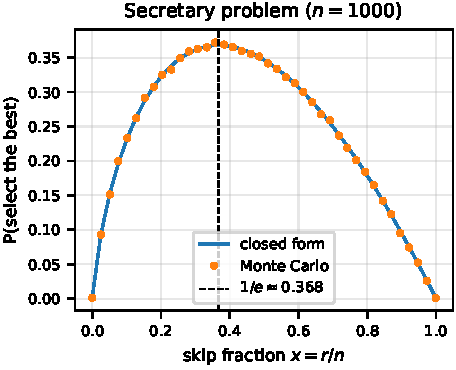
\includegraphics[width=\columnwidth]{figures/secretary_curve.pdf}
\caption{Secretary problem: Monte-Carlo success (points) matches the closed
form $-x\ln x$ (line); the optimum is at $x=1/e$.}
\label{fig:seccurve}
\end{figure}

\begin{figure}[t]
\centering
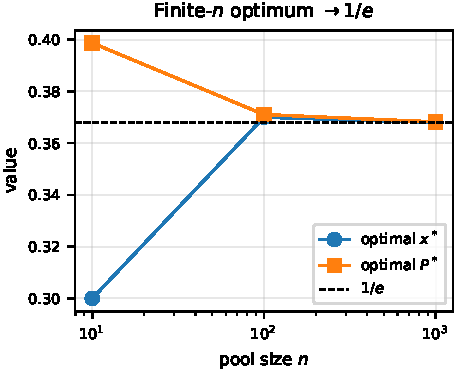
\includegraphics[width=\columnwidth]{figures/secretary_finite_n.pdf}
\caption{The optimal skip fraction $x^*$ and success $P^*$ approach $1/e$ only
as $n\to\infty$.}
\label{fig:finiten}
\end{figure}

\subsection{The 37\% rule fails on the parking problem}
Figure~\ref{fig:park} is the central result. The exact-DP optimum spends far
less than the naive rule that blindly skips the first $37\%$ of spots and then
takes the first free one. The gap widens sharply with occupancy: at
$p=\ParkPlo$ the naive rule is essentially optimal ($\ParkNaiveRegretLo\%$
regret), but at $p=\ParkPhi$ its regret explodes to $\ParkNaiveRegretHi\%$,
because when spots are usually free the right move is to hold out for the
destination itself, not to grab the first free spot after an arbitrary cutoff.

\begin{figure}[t]
\centering
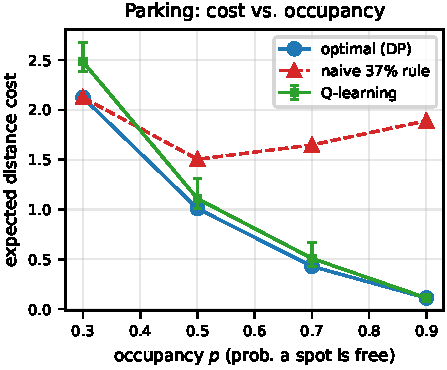
\includegraphics[width=\columnwidth]{figures/parking_cost.pdf}
\caption{Parking: expected walking cost vs.\ occupancy $p$. The learned
$Q$-agent tracks the DP optimum; the transplanted $37\%$ rule does not.}
\label{fig:park}
\end{figure}

\subsection{Search cost pulls the cutoff below 37\%}
When looking is costly, patience is penalised. Figure~\ref{fig:cost} shows the
optimal secretary cutoff falling monotonically from $1/e$ at $c=0$ to
$\CostMaxXstar$ at $c=\CostMax$: with an inspection cost, one should commit
earlier than the $37\%$ folklore suggests.

\begin{figure}[t]
\centering
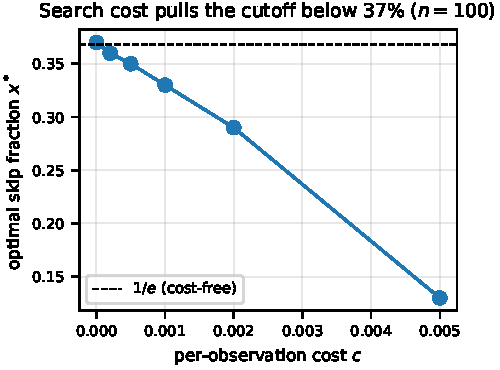
\includegraphics[width=\columnwidth]{figures/secretary_cost.pdf}
\caption{A per-observation cost pulls the optimal skip fraction below $1/e$.}
\label{fig:cost}
\end{figure}

\subsection{Agents rediscover the thresholds}
Given only rewards, tabular $Q$-learning recovers the secretary policy:
Figure~\ref{fig:agents} shows its learned cutoff concentrating near $1/e$, and
the greedy policy's exact success is within $\AgentQregret\%$ of optimal at
$n=\AgentSecN$. On parking --- the correct, per-step policy class --- it matches
the DP optimum exactly at $p=\ParkPhi$ and stays within $\ParkQregretLo\%$ in
the sparse-occupancy regime, where the acceptance boundary is hardest to pin
down from limited data. The one-parameter REINFORCE learner finds the right
secretary regime but with markedly higher variance ($\AgentReRegret\%$ regret),
and by construction cannot represent the non-stationary parking optimum ---
evidence that recovering the rule requires a policy class rich enough to hold
it.

\begin{figure}[t]
\centering
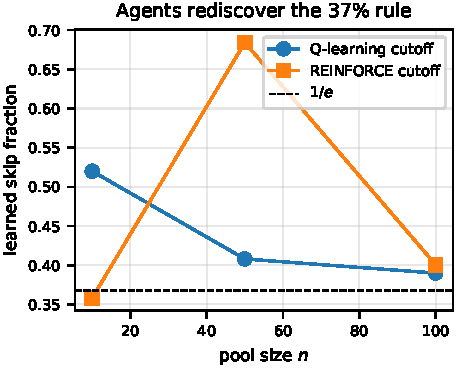
\includegraphics[width=\columnwidth]{figures/agents_secretary.pdf}
\caption{Learned skip fractions vs.\ pool size. $Q$-learning concentrates near
$1/e$; the policy-gradient cutoff is noisier.}
\label{fig:agents}
\end{figure}
